\documentclass[12pt]{article}
\newcommand{\ts}{\textsuperscript}
\usepackage[margin=1in]{geometry}
\usepackage{caption}
\usepackage{cite}
\usepackage{subcaption,graphicx}
\usepackage{lineno, blindtext}
\usepackage{float}
\usepackage{color}
\usepackage{graphicx}
\usepackage[hidelinks]{hyperref}
\usepackage{enumitem}
\usepackage{multicol}
\usepackage{fancyhdr}
\usepackage{times}
\usepackage{mathtools}
\setlength{\parindent}{0pt}
\newcommand{\forceindent}{\leavevmode{\parindent=1em\indent}}
\usepackage{amsmath}



\author{Ryan Fielding \ \ \ 301284210} 
\title{\textbf{Currency Arbitrage Optimization\\}
\bigskip
\bigskip
MSE 426 Engineering Design Optimization\\Project Report
} 
\date{April 8$^{\text{th}}$, 2020}

\begin{document}
\maketitle
\newpage
\tableofcontents
\newpage
\listoffigures
\listoftables
\newpage

\section{Introduction}
\subsection{Currency Arbitrage}
Currency arbitrage is a moderately complex optimization problem that enables banks and larger financial institutions to trade capital via a range of different currencies in order to make a gain or profit. As defined by Investopedia;
\begin{quote}
A currency arbitrage is a forex strategy in which a currency trader takes advantage of different spreads offered by brokers for a particular currency pair by making trades. Different spreads for a currency pair imply disparities between the bid and ask prices. Currency arbitrage involves buying and selling currency pairs from different brokers to take advantage of the miss priced rates. \cite{invest}
\end{quote}
Essentially, differences in two or more currency exchange rates, for example the exchange of the US dollar for the Canadian dollar, \textbf{USD2CAD}, can enable an individual to make a profit by exchange one currency for another, and back. In the case of three or more currencies, there are different combinations of trading 'routes' or 'loops' that can be taken to maximize one's proft.
\subsection{The Idea}
After completing over a year long internship in California, USA, I began to observe the trend of the \textbf{USD2CAD} exchange rate in order to maximize the value of my earnings once transferred to CAD currency. The following figure displays the rate's trend over the last 3 months.

\begin{figure}[H]
    \centering
    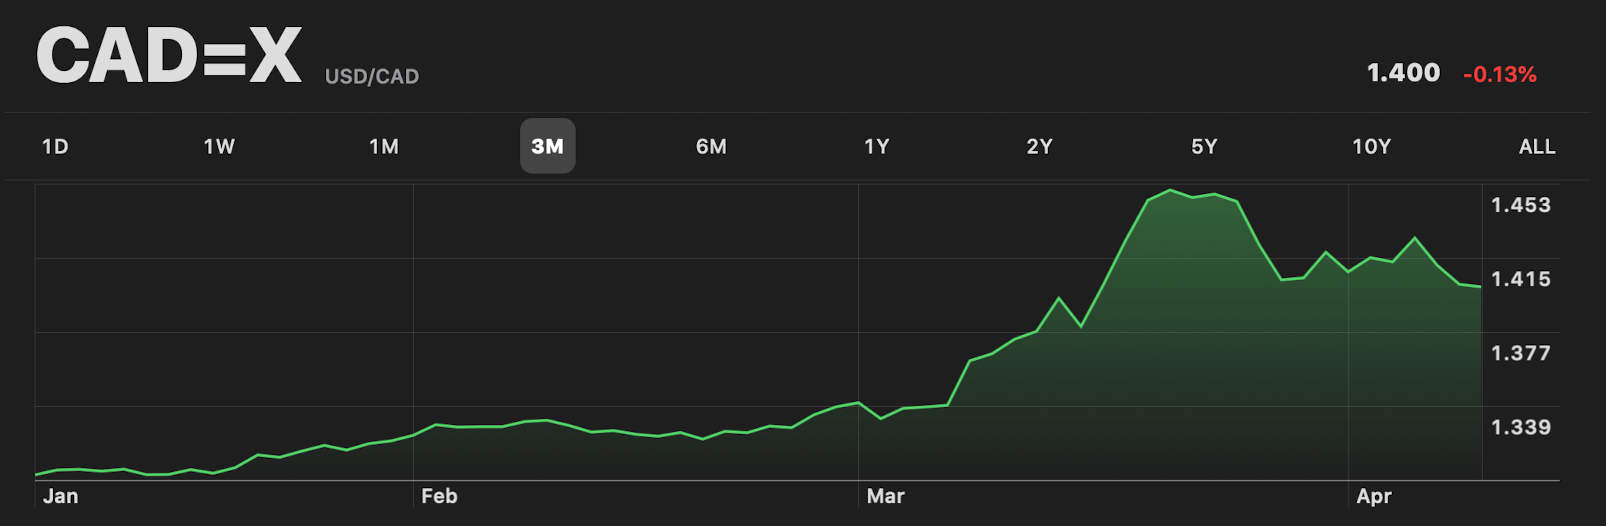
\includegraphics[width=.9\linewidth]{figures/rate}
    \caption{USD2CAD Exchange Rate, 3 Months \cite{rate}}
    \label{fig:rate}
\end{figure}

After formulating and solving the optimization problem to transfer USD to CAD, and then back to USD at a lower exchange rate, it is clear that the final amount will be the initial amount scaled by a ratio of the 2 exchange rates. However, this is too simple of a problem that only contains 4 control variables, \textbf{USD transfer amount, CAD transfer amount, rate 1, rate 2}. After some consideration, why not add another currency and find the optimal path? Thus, we have currency arbitrage.

\section{Problem Description}
Fundamentally, currency can be exchanged between the 3 currencies according to the following diagram. As shown, there are 6 links, meaning 6 exchange rates, where arrows in opposite directions are the inverses of each other. For example, going from $USD2CAD = 1.41$, and thus $CAD2USD = 1/1.41 = 0.709$. Hence, there are 3 independent exchange rates.

\begin{figure}[H]
    \centering
    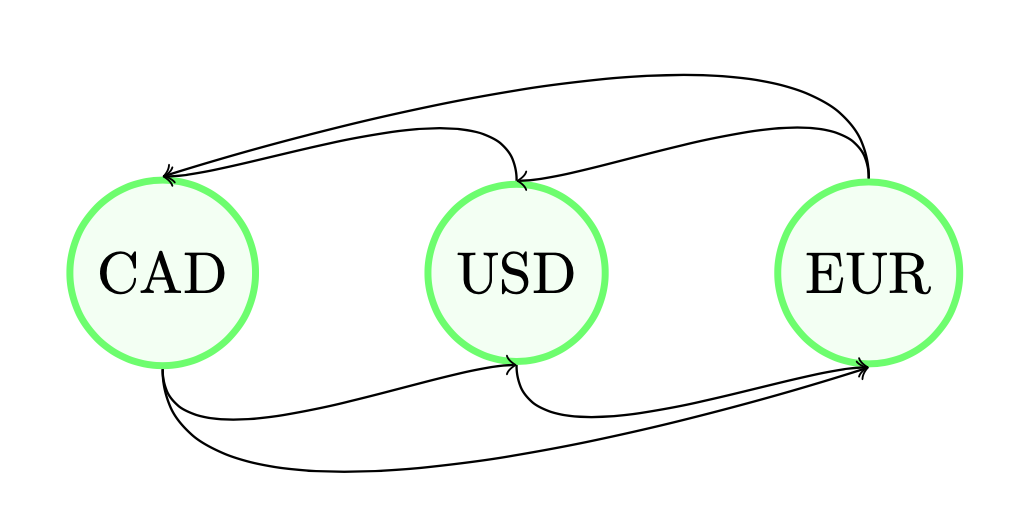
\includegraphics[width=.5\linewidth]{figures/flow}
    \caption{Arbitrage Flow}
    \label{fig:flow}
\end{figure}

\subsection{Problem Variables}
\subsubsection{2-way Arbitrage}
For simplicity, we assume a starting amount of 10, which can be in thousands, millions, etc. For the most basic problem, 2-way arbitrage, we start with the initial amount in one currency, convert it to the other currency and back again. Hence, we have 2 variables for the amounts to send. We also have 2 more variables for the rates at which to send these amounts. 
\begin{itemize}
	\item $x_{1}$ = USD to CAD transfer amount
	\item $x_{2}$ = CAD to USD transfer amount
	\item $x_{3}$ = USD to CAD transfer rate
	\item $x_{4}$ = CAD to USD transfer rate
\end{itemize}

\subsubsection{3-way Arbitrage}
To complicate the previous problem, we will add another currency, \textbf{EUR}, the Euro. One can see that this problem immediately becomes a problem of 9 variables, $n$, rather than 4. Thus, the formula for $n = (num. of currencies)^{2}$. The following table will be used to tabulate the associated transfer rates and amounts, where the \textbf{(col, row)} value represents the exchange rate \textbf{from col to row}. For example, the bottom center value of \textbf{0.9260} represents the USD2EUR exchange rate.
\begin{table}[H]
\centering
\begin{tabular}{|c|c|c|c|}
\hline 
• & CAD & USD & EUR \\ 
\hline 
CAD & 1 & 1.4113 & 1.52448 \\ 
\hline 
USD & 0.7085 & 1 & 1.0799 \\ 
\hline 
EUR & 0.6559 & 0.9260 & 1 \\ 
\hline 
\end{tabular} 
\caption{Exchange Rates}
\label{tab:rates}
\end{table}
Similarly, a table of the same format will be used for the transfer amounts from each currency to another, which are the problem variables.
\begin{table}[H]
\centering
\begin{tabular}{|c|c|c|c|}
\hline 
• & CAD & USD & EUR \\ 
\hline 
CAD & $x_{1}$ & $x_{2}$ & $x_{3}$ \\ 
\hline 
USD & $x_{4}$ & $x_{5}$ & $x_{6}$ \\ 
\hline 
EUR & $x_{7}$ & $x_{8}$ & $x_{9}$ \\ 
\hline 
\end{tabular} 
\caption{Problem Variables, 3-way}
\end{table}
The chosen rates for the solution of the problem will be selected at any given time to see if there is potential for positive gains via arbitrage. In this problem, the rates selected in table \ref{tab:rates} were pulled from an online exchange rate monitoring tracker, see \cite{xe}. This is the a common model that modern day banks use for \textbf{Arbitrage Detection}, essentially constantly checking rates across many currencies to detect potential opportunity for profit.

\subsubsection{3-way Arbitrage with Variable Rates}
Finally, one can consider what potential gains could be made off optimized exchange rates rather than those given at the current time. The encompassing question is: if the relationship between said currencies is at an optimal point, what is the point (what are the rates), and how much should be routed through each currency? The following table displays our new set of variables.
\begin{table}[H]
\centering
\begin{tabular}{|c|c|c|c|}
\hline 
• & CAD & USD & EUR \\ 
\hline 
CAD & $x_{1}$ & $x_{2}$ & $x_{3}$ \\ 
\hline 
USD & $x_{4}$ & $x_{5}$ & $x_{6}$ \\ 
\hline 
EUR & $x_{7}$ & $x_{8}$ & $x_{9}$ \\ 
\hline 
Rates & $x_{10}$ & $x_{11}$ & $x_{12}$ \\ 
\hline 
\end{tabular} 
\caption{Problem Variables, 3-way, Variable Rates}
\end{table}


\subsection{Objective Functions and Constraints}
\subsubsection{2-way Arbitrage}
Firstly, there are transaction fees associated with international bank wire transfers. They will be taken into account for this problem, but ignored for the 3-way arbitrage since they are minuscule compared to bank transfer sums. The following figure displays said transfer fees for USD and CAD transfers.
\begin{figure}[H]
    \centering
    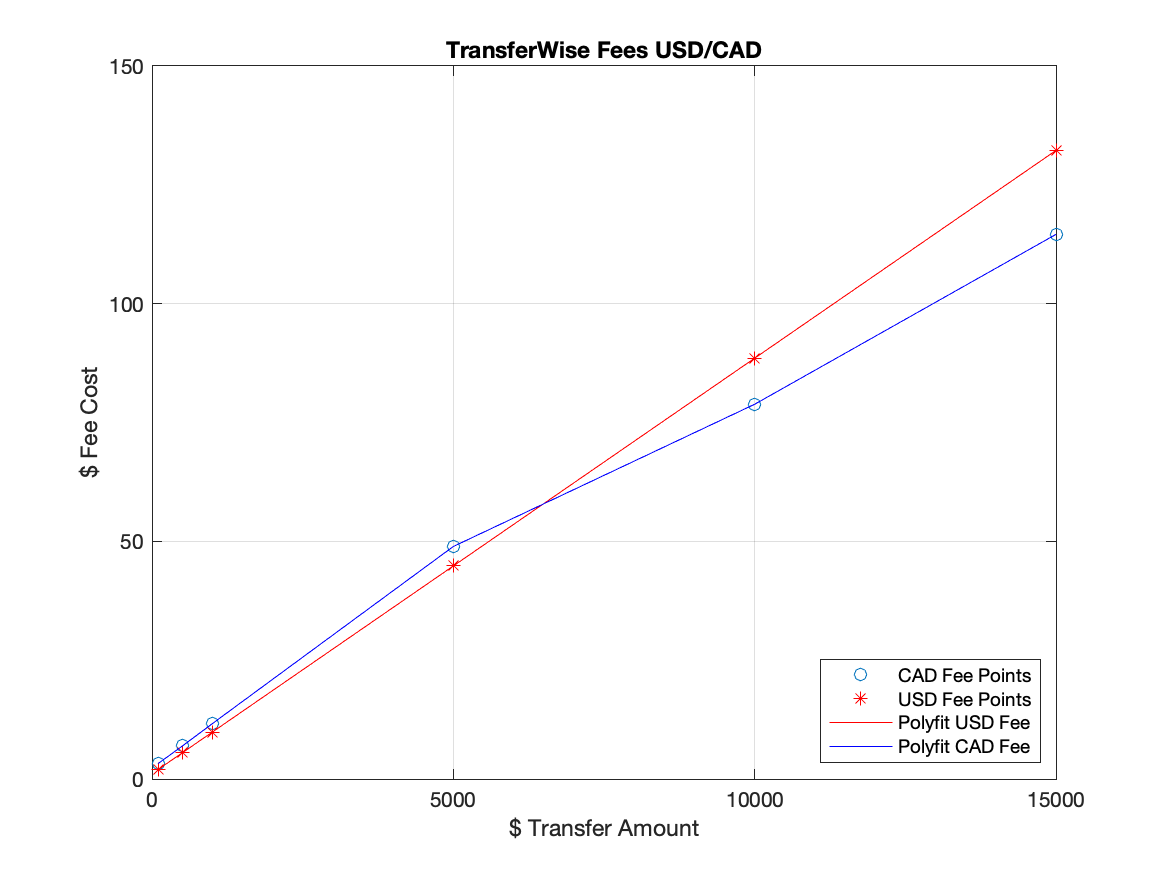
\includegraphics[width=.9\linewidth]{figures/fees.png}
    \caption{TransferWise Transfer Fees, USD and CAD \cite{tw}}
    \label{fig:tw}
\end{figure}

To begin, we set the following objective function, subject to practical constraints.
%f = -( (x(1)-usdFee(x(1)))*x(3) + (x(2) - cadFee(x(2)))/x(4) - x(1)); %in USD
%c(1)=(x(1)-usdFee(x(1)))*x(3) - x(2);
\begin{alignat}{3}
\max_x              &\quad&  f = -[ (x_{1} - usdFee(x_{1}))x_{3} + (x_{2} - cadFee(x_{2}))/x_{4} - x_{1} ]  &          & \\
\text{subject to: } &  &  x_{2} - (x_{1}-usdFee(x_{1}))x_{3}  && \quad \leq 0 &
\end{alignat}
Where \textit{usdFee()} and \textit{cadFee()} calculate the transfer fees, and the non-linear constraint (1) ensures that the amount sent back to USD from CAD, $x_{2}$, cannot be more than the amount received, $x_{1}$. Lastly, the following bounds are set, according to the 5 year high's and low's of the exchange rates for USD to CAD found on \cite{xe}, and $x_{0}$ is the initial amount of \$10,000 USD.

\begin{equation}
\begin{split}
x_{lb} & = [0, 0, 1.19588, 1.19588]\\
x_{ub} & = [x_{0}, 60000, 1.4652, 1.4652] 
\end{split}
\end{equation}

\subsubsection{3-way Arbitrage}
In this problem of 9 variables, we will neglect transaction fees, since one cannot calculate from TransferWise or other online sources the potential fees for transfers of millions of dollars. Also, we will be running the problem with $x_{0}=10$ in CAD, whether this be thousands or millions, the relative gains will be the same. The problem to be optimized is:
%f = -(x0 + (EXrates(1,2)*x(2) + EXrates(1,3)*x(3)) - (x(4) + x(7)));
%Aeq = [0 1 0 -EXrates(2,1) 0 -EXrates(2,3) 0 1 0;
   % 0 0 1 0 0 1 -EXrates(3,1) -EXrates(3,2) 0];
%beq = [0; 0];
\begin{alignat}{3}
\max_x              &\quad&  f = -(x_{0} + (EXrates(1,2)*x_{2} + EXrates(1,3)*x_{3}) - (x_{4} + x_{7}))  &          & \\
\text{subject to: } &  &  x_{2} + x_{8} - [EXrates(2,1)*x_{4} + EXrates(2,3)*x_{6}] && \quad = 0 & \\
 &  &  x_{3} + x_{6} - [EXrates(3,1)*x_{7} + EXrates(3,2)*x_{8}] && \quad = 0 & 
\end{alignat}
Our 3 by 3 matrix, \textit{EXrates}, can be seen in table \ref{tab:rates}, where elements are selected in MATLAB as \textit{EXrates(row,col)}. The two constraints listed ensure that no capital is left in the other currencies EUR and USD, inputs = outputs. The following bounds are also specified. Notice that $x_{1}, x_{5}, x_{9}$ can only be 0, similar to the diagonals of table \ref{tab:rates}, since CAD2CAD, and so forth, would be pointless.
\begin{equation}
\begin{split}
x_{lb} & = [0,0,0,0,0,0,0,0,0]\\
x_{ub} & = [0,10,10,10,0,10,10,10,0]
\end{split}
\end{equation}

\subsubsection{3-way Arbitrage with Variable Rates}
\label{xguess}
Finally, rather than using constant rates that reflect the market at only one instance in time, we will add 3 variables for said exchange rates, to find potential optimal arbitrage opportunities.  Our objective function remains the same, however the constraints are now non-linear, since elements of \textit{EXrates} all depend on $x_{10},x_{11},x_{12}$.
%f = -(x0 + (EXrates(1,2)*x(2) + EXrates(1,3)*x(3)) - (x(4) + x(7)));
\begin{alignat}{3}
\max_x &\quad  f = -(x_{0} + (EXrates(1,2)*x_{2} + EXrates(1,3)*x_{3}) - (x_{4} + x_{7}))  &\\
\text{subject to: }  &\quad\quad x_{2} + x_{8} - [EXrates(2,1)*x_{4} + EXrates(2,3)*x_{6}] &  = 0 \\
 & \quad\quad   x_{3} + x_{6} - [EXrates(3,1)*x_{7} + EXrates(3,2)*x_{8}] & = 0 \\
 & \quad\quad   -(EXrates(1,2)*x_{2} + EXrates(1,3)*x_{3}) - (x_{4} + x_{7}) & \leq 0
\end{alignat}
Constraint (11) is implemented to ensure that strictly positive gains are found, as it can be seen later in this report that \textbf{ga} finds many optima, even those with negative gains. The values of \textit{EXrates} are:
%cad2usd = x(10);
    %cad2eur = x(11);
    %usd2eur = x(12);
\begin{table}[H]
\centering
\begin{tabular}{|c|c|c|c|}
\hline 
• & CAD & USD & EUR \\ 
\hline 
CAD & 1 & 1/$x_{10}$ & 1/$x_{11}$ \\ 
\hline 
USD & $x_{10}$ & 1 & 1/$x_{12}$ \\ 
\hline 
EUR & $x_{11}$ & $x_{12}$ & 1 \\ 
\hline 
\end{tabular} 
\caption{Variable Exchange Rates}
\label{tab:ratesVar}
\end{table}
Subject to the following bounds, with rates based off the 5-year all time high's and low's found via \cite{xe}:
\begin{equation}
\begin{split}
x_{lb} & = [0,0,0,0,0,0,0,0,0,0.68250,0.61961,0.79937]\\
x_{ub} & = [0,10,10,10,0,10,10,10,0,0.83642,0.76188,0.96242]
\end{split}
\end{equation}

\section{Results and Methodology}
To solve the aforementioned problems, \textbf{MATLAB R\_2019b} will be used, with the implementation of the \textit{Optimization Toolbox} and \textit{Global Optimization Toolbox}. Primary functions used will be \textbf{fmincon} and \textbf{ga}. The results for each type of optimization algorithm run on each problem can be seen in the following sections.

\subsection{2-way Arbitrage}
Code for this solution can be seen in \textit{arb2.m}. As mentioned earlier, $x_{0}$ of \$10,000 USD will be used. The following tables outline the results.
\begin{table}[H]
    \centering
    \begin{tabular}{lllll}
Optimum & Profit & Gain & Iterations & FuncEvals \\ 
\hline 
-16577.8855 & 6577.8855 & 0.65779 & 15 & 80 \\ 
\hline 
\end{tabular}
    \caption{2-way Arbitrage - \textbf{fmincon} Results}
    \label{tab:2fm}
\end{table}

\begin{table}[H]
    \centering
    \begin{tabular}{lllll}
Optimum & Profit & Gain & Iterations & FuncEvals \\ 
\hline 
-15256.2012 & 5256.2012 & 0.52562 & 4 & 42656 \\ 
\hline 
\end{tabular}
    \caption{2-way Arbitrage - \textbf{ga} Results}
    \label{tab:2ga}
\end{table}

\begin{table}[H]
    \centering
    \begin{tabular}{lll}
X & FMOptima & GAOptima \\ 
\hline 
\$USD2CAD & 10 & 10 \\ 
\$CAD2USD & 60 & 60 \\ 
Rate USD2CAD & 1.4652 & 1.4652 \\ 
Rate CAD2USD & 1.1956 & 1.1956 \\ 
\hline 
\end{tabular}
    \caption{2-way Arbitrage Results Comparison}
    \label{tab:2res}
\end{table}
It can be seen that \textbf{fmincon} returns a gain of 66\%, whereas \textbf{ga} returns only 53\%. To summarize the results of \textbf{fmincon}, one would send \$10k USD to CAD, pay fees, at a rate of 1.4652, and then once received, send \$14,222.29 CAD back to USD at a rate of 1.1956 (see table \ref{tab:2res}). However, this is extremely impractical since those rates were seen only once in 5 years. Furthermore, \textbf{ga} does not solve as well as \textbf{fmincon} in this case, most likely because of the non linear constraint.

\subsection{3-way Arbitrage}
Code for this solution can be seen in \textit{arb3.m}. Moving forward, $x_{0}$ of 10 will be used, in CAD (see section  \ref{xguess}). The following tables outline the results. Let's assume the units are in millions, so as to acquire meaningful gains.

\begin{table}[H]
    \centering
    \begin{tabular}{lllll}
Optimum & Profit & Gain & Iterations & FuncEvals \\ 
\hline 
-10.0017 & 0.0016696 & 0.00016696 & 45 & 480 \\ 
\hline 
\end{tabular}
    \caption{3-way Arbitrage - \textbf{fmincon} Results}
    \label{tab:3fm}
\end{table}

\begin{table}[H]
    \centering
    \begin{tabular}{lllll}
Optimum & Profit & Gain & Iterations & FuncEvals \\ 
\hline 
-9.9979 & -0.0021135 & -0.00021135 & 51 & 9900 \\ 
\hline 
\end{tabular}
    \caption{3-way Arbitrage - \textbf{ga} Results}
    \label{tab:3ga}
\end{table}
Clearly, \textbf{ga} does not return a viable solution, however \textbf{fmincon} does, and yields a gain of 0.017\%, or \$1,700 CAD. Based off the selected exchange rates for this arbitrage detection, as shown in table \ref{tab:rates}, a profit can be made. How to achieve this result? See table \ref{tab:3res} below.
\begin{table}[H]
    \centering
    \begin{tabular}{lll}
X & FMOptima & GAOptima \\ 
\hline 
\$CAD2CAD & 0 & 2.0391e-17 \\ 
\$USD2CAD & 0.0010832 & 9.1614 \\ 
\$EUR2CAD & 6.561 & 8.6987 \\ 
\$CAD2USD & 9.9976 & 14.2436 \\ 
\$USD2USD & 0 & 0 \\ 
\$EUR2USD & 0.022085 & 5.8152e-14 \\ 
\$CAD2EUR & 0.00433 & 11.9491 \\ 
\$USD2EUR & 7.1061 & 0.93017 \\ 
\$EUR2EUR & 0 & 0 \\ 
\hline 
\end{tabular}
    \caption{3-way Arbitrage Results Comparison}
    \label{tab:3res}
\end{table}
Essentially, one would begin with \$10 million CAD. The row names \textbf{\$CAD2CAD,\$USD2CAD...} and so on, represent the corresponding transfer amounts. Since we start with CAD, one would send \$9.9976 to USD, and \$0.00433 to EUR, and so forth, until all currency is converted back to CAD, resulting in \$10,001,670 CAD (table \ref{tab:3fm}).

\subsection{3-way Arbitrage with Variable Rates}
Code for this solution can be seen in \textit{arb3vary.m}. Finally, as outlined in section \ref{xguess}, the optimal arbitrage transfer amounts and rates have been tabulated in the following tables. It can be noted that there are many optima for this problem. For \textbf{fmincon}, a starting point of $x_{guess} = x_{ub}$ will be used, since larger trades produce higher gains.

\begin{table}[H]
    \centering
    \begin{tabular}{lllll}
Optimum & Profit & Gain & Iterations & FuncEvals \\ 
\hline 
-18.4314 & 8.4314 & 0.84314 & 1 & 49 \\ 
\hline 
\end{tabular}
    \caption{3-way Arbitrage, Variable Rates - \textbf{fmincon} Results}
    \label{tab:3fmv}
\end{table}

\begin{table}[H]
    \centering
    \begin{tabular}{llll}
& CAD & USD & EUR \\ 
\hline 
CAD & 1 & 1.3035 & 1.433 \\ 
USD & 0.76716 & 1 & 1.1248 \\ 
EUR & 0.69786 & 0.88905 & 1 \\ 
\hline 
\end{tabular}
    \caption{3-way Arbitrage, Variable Rates - \textbf{fmincon} Exchange Rates}
    \label{tab:3fmrv}
\end{table}

\begin{table}[H]
    \centering
    \begin{tabular}{lllll}
Optimum & Profit & Gain & Iterations & FuncEvals \\ 
\hline 
-10.1785 & 0.17846 & 0.017846 & 54 & 534856 \\ 
\hline 
\end{tabular}
    \caption{3-way Arbitrage, Variable Rates - \textbf{ga} Results}
    \label{tab:3gav}
\end{table}

\begin{table}[H]
    \centering
    \begin{tabular}{llll}
& CAD & USD & EUR \\ 
\hline 
CAD & 1 & 1.3856 & 1.3129 \\ 
USD & 0.72171 & 1 & 1.212 \\ 
EUR & 0.76164 & 0.82512 & 1 \\ 
\hline 
\end{tabular}
    \caption{3-way Arbitrage, Variable Rates - \textbf{ga} Exchange Rates}
    \label{tab:3garv}
\end{table}
Tables \ref{tab:3fmv} to \ref{tab:3garv} display the optimization results for this problem. Clearly, there exist much higher potential arbitrage gains, 84\% and 24\% from \textbf{fmincon} and \textbf{ga}, respectively. After a quick investigation of tables \ref{tab:3fmrv} and \ref{tab:3garv}, we can see that such rates are fairly impractical. A discussion of practicality is outlined in section \ref{prac}. The aforementioned optimum occur at the following design points.
\begin{table}[H]
    \centering
    \begin{tabular}{lll}
X & FMOptima & GAOptima \\ 
\hline 
\$CAD2CAD & 0 & 5.5656e-15 \\ 
\$USD2CAD & 8.6448 & 6.1336 \\ 
\$EUR2CAD & 3.0701 & 7.8659 \\ 
\$CAD2USD & 8.6907 & 9.7849 \\ 
\$USD2USD & 0 & 6.0369e-17 \\ 
\$EUR2USD & 6.8464 & 0.4752 \\ 
\$CAD2EUR & 7.2982 & 8.7733 \\ 
\$USD2EUR & 5.4509 & 2.1588 \\ 
\$EUR2EUR & 0 & 0 \\ 
Rate CAD2USD & 0.72409 & 0.79793 \\ 
Rate CAD2EUR & 0.70343 & 0.71186 \\ 
Rate USD2EUR & 0.87742 & 0.97601 \\ 
\hline 
\end{tabular}
    \caption{3-way Arbitrage, Variable Rates Results Comparison}
    \label{tab:3resv}
\end{table}
It is interesting to see that \textbf{fmincon} finds a solution in which all transfer amounts = \$9.01, and only the rates vary. This is of course different with other trials where $x_{guess}$ is changed. Finally, it was noted that since there are numerous optima, \textbf{ga} was run 20 times to observe the many optima and analyse the highest few for better understanding of practicality.
\begin{table}[H]
    \centering
    \begin{tabular}{lllllll}
Data & Run1 & Run2 & Run3 & Run4 & Run5 & Run6 \\ 
\hline 
Optimum & -10.41 & -13.9648 & -11.4928 & -13.132 & -11.0421 & -11.942 \\ 
\$CAD2CAD & 0 & 0 & 0 & 0 & 0 & 0 \\ 
\$USD2CAD & 1.2831 & 9.6016 & 9.9705 & 9.9171 & 3.8731 & 7.2703 \\ 
\$EUR2CAD & 2.3346 & 2.6524e-06 & 4.2076 & 0.13599 & 1.545 & 3.4577 \\ 
\$CAD2USD & 2.9045 & 0.10344 & 8.6387 & 3.0051 & 0.84417 & 3.7953 \\ 
\$USD2USD & 0 & 0 & 0 & 0 & 0 & 0 \\ 
\$EUR2USD & 0.45489 & 8.3484 & 7.219 & 8.3351 & 8.1373 & 5.6448 \\ 
\$CAD2EUR & 1.9874 & 10 & 9.9999 & 8.5721 & 5.8258 & 9.4535 \\ 
\$USD2EUR & 1.6189 & 0.91275 & 4.5486 & 2.4013 & 6.0411 & 2.3746 \\ 
\$EUR2EUR & 0 & 0 & 0 & 0 & 0 & 0 \\ 
Rate CAD2USD & 0.83642 & 0.6825 & 0.6825 & 0.6825 & 0.68251 & 0.6825 \\ 
Rate CAD2EUR & 0.61961 & 0.76188 & 0.76188 & 0.76081 & 0.75835 & 0.76188 \\ 
Rate USD2EUR & 0.96242 & 0.79937 & 0.83718 & 0.8118 & 0.87142 & 0.80016 \\ 
\hline 
\end{tabular}
    \caption{3-way Arbitrage, Variable Rates GA Runs}
    \label{tab:gaTrials}
\end{table}
Clearly there are many solutions that all yield very high gains with the highest being 39.6\% (Run2). The genetic algorithm is able to remain within the constraints and ensure all money is converted back to CAD, while obtaining different levels of profit for different transactions and exchange rates.

\section{Conclusion}
A significant amount of understanding of currency arbitrage, as well as different optimization algorithms, has been gained throughout the duration of this project. Not only through the many solutions produced, but the implementation of the objective functions, their constraints, linear and non linear, and finally upper and lower bounds, have induced a great deal of learning concerning engineering design optimization.  To list the outcomes:
\begin{itemize}
	\item An in depth understanding of currency arbitrage and it's complexity.
	\item The constraints and drawbacks to currency arbitrage.
	\item The many different optimization algorithms, and their pros and cons.
	\item A valid assessment of arbitrage detection and it's potential in the market.
	\item 2-way arbitrage (in this report) can provide gains with tangible income, assuming proper monitoring of exchange rates.
	\item A sound understanding of practicality or the market.
\end{itemize}
Not only engineering specific applications, but the concept as a whole, as proven through this report in the field of Investment Banking and economy. Optimization can be applied to many different fields and problems.
\subsection{Practicality}
\label{prac}
To better understand how practical this information is, let's recall the optima shown in table \ref{tab:gaTrials}. After just 6 trials, and minimal tuning of the genetic algorithm due to project time constraints, a few profitable solutions were found. An in depth analysis of the selected exchange rates deems whether or not a solution is practical. In practice, these optima on their own are not practical, since there is a slim chance that the market rates will ever actually equate to these optima. However, 2 potential ideas are discussed below.
\subsubsection{Brute Force Method}
A simple solution would be to run the genetic algorithms over thousands of iterations to produce numerous optima, and to consistently monitor the market rates in real time. If these rates were to ever connect, an immediate series of transactions could lead to the estimated profit.
\subsubsection{Rate Correlation}
There are many theories and analyses that prove positive and negative correlation between exchange rates \cite{corr}. A proper implementation of this idea could increase the practicality of this arbitrage optimization problem. Specifically, by varying the third rate subject to past market correlation data, while dependant on CAD2USD and CAD2EUR rates. Thus, any proposed solutions could have a higher possibility of ever equating to real time market rates.\\\\\\
All development can be seen on Github \cite{ry}.

\newpage
% ADD BIBLIOGRAPHY
\nocite{*}
\bibliographystyle{IEEE/IEEEtran}
\bibliography{IEEE/IEEEabrv,IEEE/biblio}


\end{document}